\chapter{Introducción específica}

\label{Chapter2}

Este capítulo presenta las tecnologías de hardware y de software de terceros que sustentan el prototipo de telemetría. Se describe qué componentes se utilizaron, para qué sirven y qué capacidades ofrecen según la documentación del fabricante. La asignación de periféricos, la interconexión en el prototipo, la arquitectura de firmware y el dispositivo móvil se desarrollan en el capítulo~\ref{Chapter3}.

%----------------------------------------------------------------------------------------
\section{Plataforma de hardware}
\label{sec:plataforma-hardware}

La plataforma de desarrollo seleccionada fue la placa NUCLEO-F446RE \citep{st_nucleo_f446re}, que integra el microcontrolador STM32F446RET6 en encapsulado LQFP64 \citep{st_stm32f446re}. El núcleo es un procesador ARM Cortex-M4 con unidad de punto flotante y periféricos orientados a adquisición de datos, temporización y comunicación serie.

Según la documentación del fabricante, el STM32F446RET6 admite frecuencias de reloj de hasta 180MHz y dispone de controladores USART (del inglés \textit{Universal Synchronous/Asynchronous Receiver Transmitter}), I2C (del inglés \textit{Inter-Integrated Circuit}), SPI (del inglés \textit{Serial Peripheral Interface}), acceso directo a memoria (DMA, del inglés \textit{Direct Memory Access}), temporizadores de propósito general y un IWDG (del inglés \textit{Independent Watchdog}). En la placa NUCLEO-F446RE se integra un depurador ST-LINK con puerto serie virtual, habitual en etapas de depuración. En la figura~\ref{fig:nucleo-f446re} se muestra la placa de desarrollo empleada.

\begin{figure}[H]
	\centering
	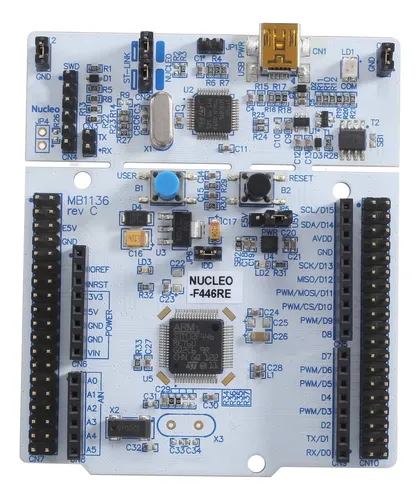
\includegraphics[width=0.72\textwidth]{Figures/nucleo-f446re.png}
	\caption[Placa NUCLEO-F446RE]{Placa de desarrollo NUCLEO-F446RE \citep{st_nucleo_f446re}.}
	\label{fig:nucleo-f446re}
\end{figure}

La elección de esta familia se fundamentó en la disponibilidad de varios buses serie en los conectores de prototipado, la compatibilidad con middleware publicado por STMicroelectronics y la documentación de referencia para la línea STM32F4. El STM32F446RET6 posee 512KiB de memoria flash y 128KiB de SRAM, varias instancias USART, I2C y SPI operables en paralelo, y un margen de frecuencia de reloj adecuado para sostener adquisición multicanal sin saturar el procesador. La placa NUCLEO-F446RE expone esos periféricos mediante los conectores Arduino y Morpho y deja margen de expansión respecto del conjunto previsto para el prototipo.

\subsection{Herramientas de desarrollo y depuración}

Además, la plataforma se complementa con el ecosistema STM32Cube de STMicroelectronics. STM32CubeMX es la utilidad gráfica para definir pines, relojes e instancias de periféricos en el microcontrolador. STM32CubeIDE \citep{st_stm32cubeide} agrupa el editor de código, el depurador y el compilador cruzado GNU para ARM (\texttt{arm-none-eabi-gcc}). Ambas herramientas permiten generar y mantener proyectos basados en la capa HAL.

%----------------------------------------------------------------------------------------
\section{Componentes y módulos externos}
\label{sec:componentes-externos}

El prototipo incorpora módulos de adquisición, comunicación y almacenamiento cableados al microcontrolador: receptor GNSS \citep{gnss_overview}, unidad inercial de seis ejes, transceptor Bluetooth de baja energía y tarjeta microSD. Esos periféricos usan buses serie del tipo UART (del inglés \textit{Universal Asynchronous Receiver Transmitter}), I2C y SPI. En la tabla~\ref{tab:componentes-externos} se resume la función de cada elemento y el tipo de interfaz física que expone.

\begin{table}[H]
	\centering
	\caption[Módulos del prototipo]{Módulos externos del prototipo y su función.}
	\setlength{\tabcolsep}{4pt}
	\begin{tabularx}{\textwidth}{@{}>{\raggedright\arraybackslash}p{2.2cm}>{\raggedright\arraybackslash}p{3.2cm}>{\raggedright\arraybackslash}p{2.8cm}>{\raggedright\arraybackslash}X@{}}
		\toprule
		\textbf{Módulo} & \textbf{Función} & \textbf{Interfaz física} & \textbf{Características relevantes} \\
		\midrule
		NEO-M8N & Posicionamiento GNSS & UART & Salida de tramas en formato NMEA. Alimentación 3.3V típica \citep{ublox_neo_m8n} \\
		LSM6DSO & Medición inercial (6 ejes) & I2C & Acelerómetro y giroscopio integrados. Dirección I2C configurable \citep{st_lsm6dso} \\
		HC-10 (BT05) & Enlace Bluetooth & UART & Módulo transparente hacia un controlador BLE en el extremo móvil \citep{hc10_bt05} \\
		Tarjeta microSD & Memoria removible & SPI & Soporta sistemas de archivos FAT en aplicaciones embebidas \\
		\bottomrule
	\end{tabularx}
	\label{tab:componentes-externos}
\end{table}

El receptor NEO-M8N \citep{ublox_neo_m8n} es un módulo GNSS orientado a navegación y registro de posición. Entrega sentencias en formato NMEA \citep{nmea_0183}, estándar ampliamente difundido para intercambio de datos de posicionamiento y tiempo. En la figura~\ref{fig:neo-m8n-modulo} se ilustra el módulo empleado.

\begin{figure}[H]
	\centering
	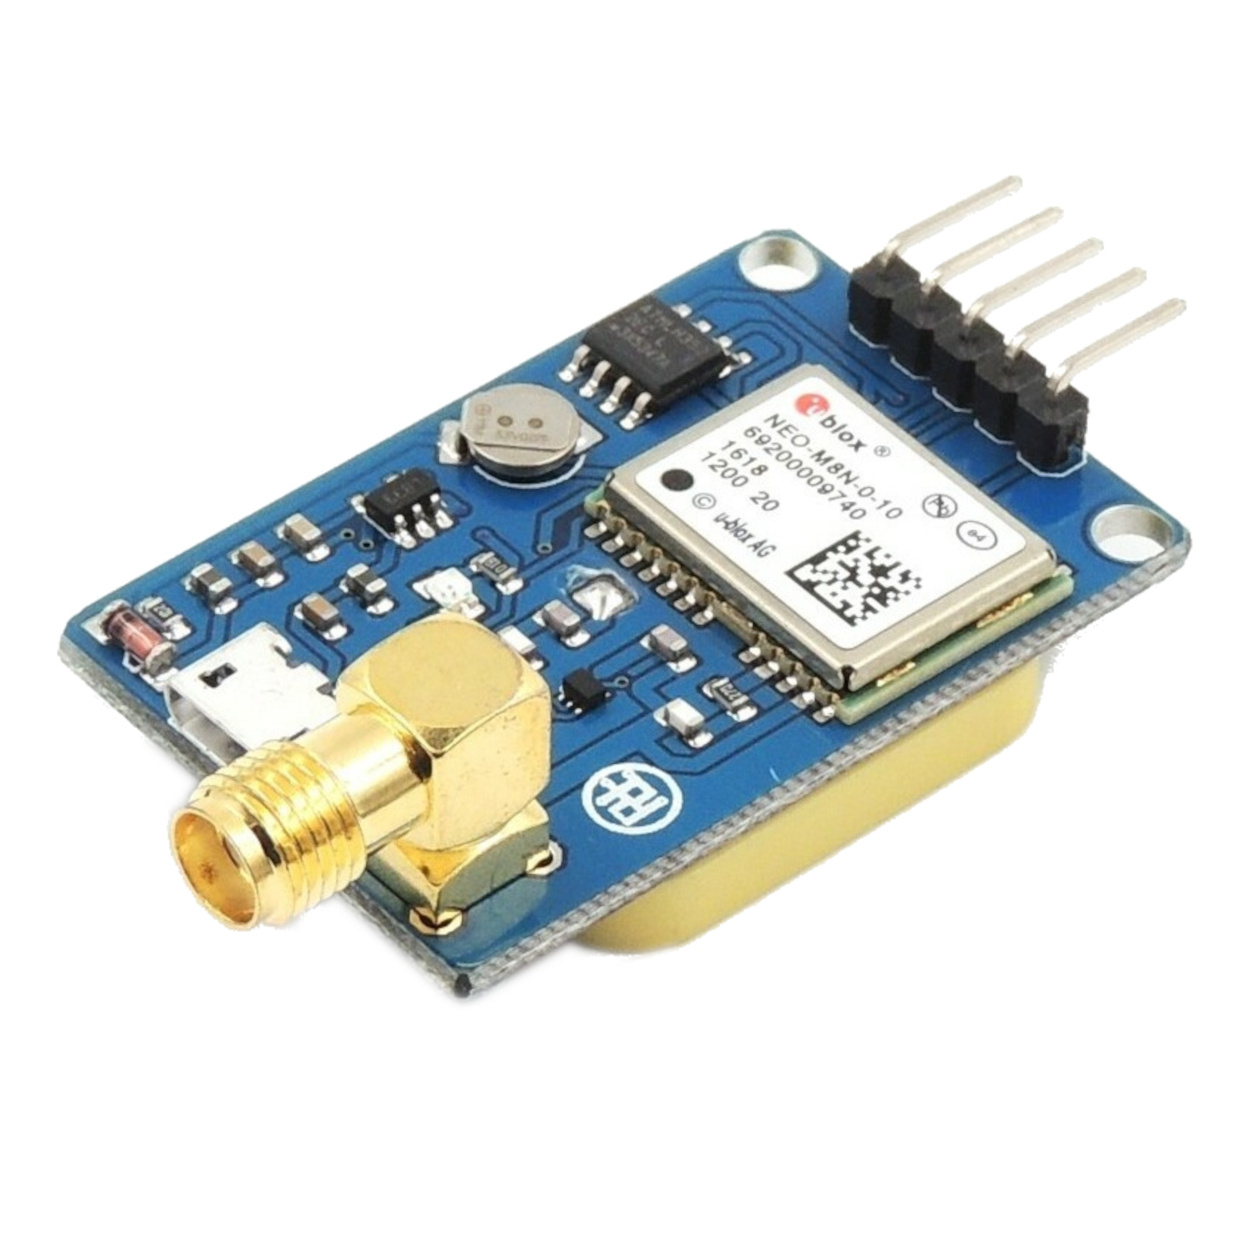
\includegraphics[width=0.55\textwidth]{Figures/neo-m8n.jpg}
	\caption[Módulo NEO-M8N]{Módulo GNSS NEO-M8N \citep{ublox_neo_m8n}.}
	\label{fig:neo-m8n-modulo}
\end{figure}

La unidad LSM6DSO \citep{st_lsm6dso} integra acelerómetro y giroscopio triaxiales en un único encapsulado. Permite obtener aceleración lineal y velocidad angular mediante lecturas de registros internos por bus I2C. En la figura~\ref{fig:lsm6dso-modulo} se ilustra el sensor empleado.

\begin{figure}[H]
	\centering
	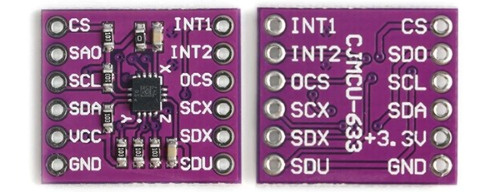
\includegraphics[width=0.68\textwidth]{Figures/lsm6dso.jpg}
	\caption[Sensor inercial LSM6DSO]{Unidad inercial LSM6DSO \citep{st_lsm6dso}.}
	\label{fig:lsm6dso-modulo}
\end{figure}

El módulo HC-10 (variante BT05 sobre CC2541) \citep{hc10_bt05} se enlaza al microcontrolador por UART. El enlace Bluetooth de baja energía con el teléfono lo gestiona el propio módulo, de modo que el host embebido puede limitarse a enviar y recibir octetos por ese puerto sin implementar el protocolo BLE en software. En la figura~\ref{fig:hc10-modulo} se ilustra el módulo empleado.

\begin{figure}[H]
	\centering
	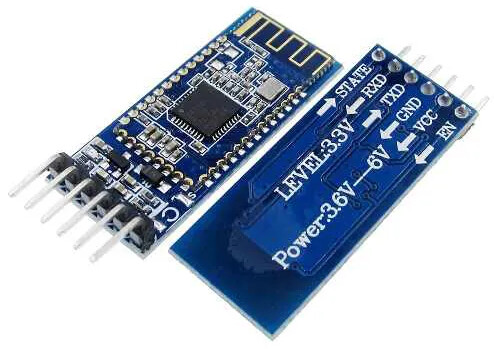
\includegraphics[width=0.55\textwidth]{Figures/hc-10.jpeg}
	\caption[Módulo HC-10]{Módulo de enlace Bluetooth HC-10 (BT05) \citep{hc10_bt05}.}
	\label{fig:hc10-modulo}
\end{figure}

La tarjeta microSD se emplea como medio de almacenamiento masivo removible. En aplicaciones embebidas suele conectarse por bus SPI y utilizarse junto con un middleware de sistema de archivos FAT que administra el contenido en bloques.

%----------------------------------------------------------------------------------------
\section{Sistema operativo y middleware}
\label{sec:rtos-middleware}

En aplicaciones embebidas con múltiples actividades concurrentes se emplean sistemas operativos de tiempo real (RTOS, del inglés \textit{Real-Time Operating System}). FreeRTOS \citep{freertos} es un núcleo de este tipo, integrado habitualmente en el árbol de middleware de STM32Cube, con planificación preemptiva y primitivas de sincronización.

\subsection{Capas de software de terceros}

Sobre el RTOS y el hardware se apoyan las siguientes piezas de soporte:

\begin{itemize}
	\item CMSIS y HAL de STM32, generados desde STM32CubeMX a partir del paquete de firmware STM32Cube para la familia F4, para abstraer GPIO, temporizadores, DMA y periféricos serie.
	\item FreeRTOS, con APIs de tareas, colas, semáforos y temporizadores de software.
	\item FatFs \citep{chan_fatfs}, middleware de sistema de archivos para memorias con formato FAT32.
	\item En el host, Ceedling \citep{ceedling} y Unity \citep{unity} para pruebas unitarias de firmware, sin formar parte del binario embarcado.
\end{itemize}

La capa HAL expone rutinas de configuración y tipos comunes para UART, I2C y SPI. CMSIS define vectores de interrupción y características del núcleo Cortex-M. FatFs proporciona funciones de alto nivel para crear, abrir y escribir archivos sobre una partición FAT.

\subsection{Stack web en el teléfono móvil}

En el extremo móvil intervienen tecnologías web estándar. Una aplicación web progresiva (PWA, del inglés \textit{Progressive Web App}) \citep{mdn_pwa} permite desplegar una interfaz en el navegador con comportamiento cercano al de una aplicación nativa. React \citep{react} es una biblioteca para construir interfaces por componentes, y Vite \citep{vite} una herramienta de empaquetado y servidor de desarrollo para el ecosistema JavaScript.

La API Web Bluetooth \citep{w3c_web_bluetooth} del navegador habilita la comunicación con periféricos BLE desde una página web, sin publicar un binario en las tiendas. Para mapas interactivos se emplean bibliotecas como Leaflet \citep{leaflet}. El diseño concreto del dispositivo móvil, el flujo de datos y la integración con el módulo HC-10 se describen en el capítulo~\ref{Chapter3}.

%----------------------------------------------------------------------------------------
\section{Protocolos y buses de comunicación}
\label{sec:protocolos-buses}

Los módulos descritos en la sección~\ref{sec:componentes-externos} se conectan al microcontrolador mediante tres interfaces serie ampliamente adoptadas en sistemas embebidos. A continuación se resume el funcionamiento de cada bus a nivel conceptual. La elección de instancias, velocidades y pines en el prototipo se documenta en el capítulo~\ref{Chapter3}.

\subsection{UART}

La comunicación UART envía y recibe octetos de forma asíncrona entre dos extremos. No comparte una línea de reloj global: ambos lados deben acordar de antemano la velocidad en baudios, el formato de trama y la polaridad de las señales. El esquema suele ser punto a punto, de modo que un puerto del microcontrolador atiende a un periférico.

\subsection{Bus I2C}

El bus I2C organiza el intercambio en torno a un maestro y uno o más esclavos sobre un par de líneas compartidas de datos y reloj. Cada esclavo se distingue por una dirección de siete u once bits anunciada en el inicio de la transferencia. Las velocidades típicas son inferiores a las del SPI, pero el cableado resulta compacto y admite varios dispositivos en el mismo bus con pines adicionales de control cuando el hardware lo exige. El maestro accede a cada periférico mediante lectura y escritura de registros internos, un esquema habitual en sensores digitales y en módulos inerciales de baja y media tasa de muestreo.

\subsection{Bus SPI}

El bus SPI opera en modo maestro-esclavo con señales dedicadas de reloj, datos de ida y vuelta y una línea de selección por cada esclavo. La sincronización la marca el reloj generado por el maestro, lo que permite alcanzar mayores velocidades de transferencia que en I2C. Un mismo bus puede alimentar varios esclavos si cada uno dispone de su señal de \textit{chip select} y solo un integrado permanece activo por intervalo de intercambio.